\section{Static APK Forensics and Natural Experiment}
\label{sec:apk}

Live chat logs cannot show what an application reads off the handset in the background. To inspect client telemetry directly, we analyzed all five audited Indian Android APKs using a deterministic ZIP, binary AXML, and DEX/Hermes byte parser (\texttt{tools/audit\_apks.py}), after resolving an earlier interrupted transfer of \texttt{AstroSage AI.apk}. Table~\ref{tab:apks} contrasts all five binaries across native Kotlin/Java and React Native stacks.

\begin{table*}[t]
\centering
\caption{Static binary forensic summary across all five audited Indian astrology APKs.}
\label{tab:apks}
\footnotesize
\setlength{\tabcolsep}{3.5pt}
\begin{tabularx}{\textwidth}{@{}L{3.25cm} L{1.50cm} L{1.65cm} L{1.45cm} c c Y@{}}
\toprule
\textbf{APK / Package ID} & \textbf{Version (Code)} & \textbf{Size (Files)} & \textbf{Stack} & \textbf{\texttt{<queries>}} & \textbf{Uniq.} & \textbf{Key Manifest, Asset \& Backend Findings} \\
\midrule
\texttt{Astrotalk.apk}\newline\nolinkurl{com.astrotalk} & \texttt{1.1.545} (545) & 89.91~MB (7,825) & Native (7~DEX) & 823 & \textbf{804} & \texttt{QUERY\_ALL\_PACKAGES=False}; \nolinkurl{apppackges.json} [sic] (\textbf{787/787} in \texttt{<queries>}); \texttt{ExternalPackageTracker} $\rightarrow$ \nolinkurl{user/apps/installed} \& \nolinkurl{save/user-upi-apps} \\
\texttt{Pandit Ji.apk}\newline\nolinkurl{com.astrology.panditji} & \texttt{1.1.421} (421) & 97.03~MB (7,119) & Native (6~DEX) & 26 & 26 & 6,193 shared paths (86.99\%) \& 3,172 identical files vs.\ Astrotalk; 1,470 \texttt{astrotalk} DEX strings; zero tracker \\
\texttt{AstroSage AI.apk}\newline\nolinkurl{com.ojassoft.astrosage} & \texttt{32.6} (1244) & 76.56~MB (4,888) & Native (6~DEX) & 23 & 23 & Zero installed-app catalog; Razorpay/Paytm/PhonePe SDKs; legacy \texttt{http://} + \texttt{https://astrosage.com} URLs \\
\texttt{Reva.apk}\newline\nolinkurl{in.mohalla.reva} & \texttt{2026.24.2} (2026242) & 38.41~MB (1,500) & RN Hermes (5~DEX) & 83 & 83 & \texttt{DETECT\_SCREEN\_CAPTURE=True}; \nolinkurl{/payments-api-gateway/v1/subscriptions/}; \nolinkurl{revaastro.in} \\
\texttt{AstroTime.apk}\newline\nolinkurl{com.theastrotime} & \texttt{4.1.8} (47) & 25.76~MB (1,315) & RN Hermes (2~DEX) & 9 & 9 & Independent RN codebase (\nolinkurl{apis.theastrotime.com}, \nolinkurl{posthog.theastrotime.com}, \nolinkurl{livekit.io}) \\
\bottomrule
\end{tabularx}
\end{table*}

\subsection{How Astrotalk Profiles Devices Without \texttt{QUERY\_ALL\_PACKAGES}}
In \texttt{Astrotalk.apk} (\texttt{v1.1.545}, code 545, SHA-256 prefix \texttt{527331d1c60a953c}), the manifest omits Google Play's restricted \texttt{QUERY\_ALL\_PACKAGES} permission completely. Instead, it embeds \textbf{823 \texttt{<package>} declarations} (804 unique package IDs after accounting for 19 merged SDK overlaps) plus 14 \texttt{<intent>} entries inside \texttt{<queries>}.

Inside \nolinkurl{assets/apppackges.json}~[sic] (63,591 bytes), we uncovered an explicit JSON target catalog containing \textbf{787 distinct} \texttt{\{"name", "package\_name"\}} objects. Cross-checking the JSON catalog against \texttt{AndroidManifest.xml} confirms exact set inclusion:
\[
|\mathcal{P}_{\mathrm{JSON}}|=787,\; |\mathcal{Q}_{\mathrm{AT}}|=804,\; |\mathcal{P}_{\mathrm{JSON}} \cap \mathcal{Q}_{\mathrm{AT}}|=787\;(100.0\%).
\]
All 17 remaining entries in $\mathcal{Q}_{\mathrm{AT}} \setminus \mathcal{P}_{\mathrm{JSON}}$ are standard payment, login, messaging, and map dependencies (\nolinkurl{com.otpless.app}, \nolinkurl{com.whatsapp}, \nolinkurl{com.paytm.pgsdk...}, \nolinkurl{com.android.chrome}, \nolinkurl{com.google.android.apps.maps}, etc.). Synchronizing \texttt{<queries>} with \nolinkurl{apppackges.json} lets \texttt{Astrotalk} query all 787 target packages through Android~11+ visibility filters without filing a Google Play \texttt{QUERY\_ALL\_PACKAGES} justification.

Bytecode inspection of \texttt{classes3.dex} traces the execution pipeline cleanly (Figure~\ref{fig:pipeline}) despite R8 class minification (\nolinkurl{Lcom/astrotalk/utils/u0;} retaining debug source \texttt{ExternalPackageTracker.kt}):
\begin{enumerate}[leftmargin=*,itemsep=2pt,topsep=3pt]
\item \textbf{Trigger:} \texttt{AuthViewModel\$\allowbreak check\allowbreak External\allowbreak Packages\$1} calls \texttt{AuthRepositoryImpl\$\allowbreak check\allowbreak External\allowbreak Packages\$2}, invoking \texttt{External\allowbreak Package\allowbreak Tracker\$\allowbreak trackIfNeeded\$1}.
\item \textbf{Cooldown \& Enumeration:} The tracker checks a \texttt{SharedPreferences} flag (\texttt{"execute\_24h\_check"}), reads \nolinkurl{assets/apppackges.json}, calls \nolinkurl{PackageManager.getInstalledPackages()}, and populates \nolinkurl{com.astrotalk.models.externalPackage.App} objects inside \texttt{getInstalledTrackedApps\$1} and \texttt{trackInstalledPackages\$1}/\texttt{\$3}.
\item \textbf{Exfiltration Endpoints:} Retrofit service interface \nolinkurl{com.astrotalk.controller.b} uploads detected packages via \texttt{S3} (\nolinkurl{@POST("user/apps/installed")} carrying \texttt{@Header("id")}, \texttt{@Header("Authorization")}, \texttt{@Query("device\_id")}, and \texttt{@Body List}), alongside companion method \texttt{O1} (\nolinkurl{@POST("/AstrotalkPayments/user/save/user-upi-apps")} via \texttt{PostSaveUser\allowbreak UpiInstalled\allowbreak AppsRequestDto}).
\end{enumerate}

\begin{figure}[t]
\centering
\resizebox{\columnwidth}{!}{%
\begin{tikzpicture}[
  node distance=5mm and 6mm,
  box/.style={draw=accentblue, rounded corners=2pt, fill=accentblue!6, text width=3.20cm, align=center, font=\scriptsize, inner sep=4.5pt},
  warn/.style={draw=alertred, rounded corners=2pt, fill=alertred!7, text width=3.30cm, align=center, font=\scriptsize, inner sep=4.5pt},
  arr/.style={-{Latex[length=2mm]}, thick, color=slategray}
]
\node[box] (json) {\texttt{assets/apppackges.json}\\(787 target apps)};
\node[box, below=of json] (man) {\texttt{AndroidManifest.xml}\\(\texttt{<queries>}: 804 unique,\\no \texttt{QUERY\_ALL\_PACKAGES})};
\node[box, right=of json, yshift=-6.5mm] (u0) {\texttt{ExternalPackageTracker}\\(\texttt{u0}, \texttt{execute\_24h\_check},\\Android \texttt{PackageManager})};
\node[warn, right=of u0] (post) {\texttt{POST user/apps/installed}\\(\texttt{b.S3} + \texttt{save/user-upi-apps})};
\draw[arr] (json.east) -- (u0.west);
\draw[arr] (man.east) -- (u0.west);
\draw[arr] (u0.east) -- (post.west);
\end{tikzpicture}%
}
\caption{Client-side device package discovery and upload chain verified inside \texttt{Astrotalk.apk} (\texttt{v1.1.545}, \texttt{classes3.dex}).}
\label{fig:pipeline}
\end{figure}

\subsection{Domain Breakdown of the 787 Targeted Applications}
Classifying all 787 entries cleanly shows what kind of user state \texttt{Astrotalk} looks for (Figure~\ref{fig:taxonomy}). Beyond broad e-commerce/travel spending proxies (189 apps), OTT streaming/news (90), health/wearables (34), exam/job search portals (26), devotional apps (18), and commuter rail (4), the payload zeroes in on high-intent financial and personal vulnerability signals:
\begin{itemize}[leftmargin=*,itemsep=1.5pt,topsep=2pt]
\item \textbf{Financial Liquidity \& Risk:} 113 banking, UPI, and diaspora remittance apps (e.g., \texttt{Google Pay}, \texttt{Paytm}, \texttt{PhonePe}, \texttt{YONO SBI}, Wise, Revolut), 38 stock and crypto platforms (\texttt{Zerodha Kite}, \texttt{Groww}, \texttt{Upstox}, \texttt{INDWealth}, Binance, WazirX), 36 consumer loan, BNPL, and gold-loan apps (\texttt{Moneyview}, \texttt{CASHe}, \texttt{iMuthoot}, \texttt{Rupeek}, CIBIL, Paisabazaar), and 49 real-money gambling and betting apps (\texttt{WinZO}, \texttt{Zupee}, \texttt{Dream11}, \texttt{1xBet}, Bet365).
\item \textbf{Intimate, Health, Labor \& AI Proxies:} 46 dating, matrimony, and live-chat apps (\texttt{Tinder}, \texttt{Bumble}, \texttt{Hinge}, Shaadi, BharatMatrimony), \textbf{16 reproductive health, pregnancy, and therapy apps} (\texttt{Flo}, Clue, Premom, \texttt{BetterHelp}, \texttt{Talkspace}), \textbf{9 gig-worker driver/delivery apps} (\texttt{Uber Driver}, Ola Driver, Rapido Captain, Swiggy/Zomato Delivery), \textbf{8 Indian government identity/welfare apps} (\texttt{DigiLocker}, mAadhaar, \texttt{PMKISAN GoI}, \texttt{Digi Yatra}), \textbf{8 AI assistants} (\texttt{ChatGPT}, Gemini, Claude, Perplexity, DeepSeek), and \textbf{103 rival astrology/tarot apps} (including its own sister package \texttt{com.astrology.panditji}).
\end{itemize}

\begin{figure*}[t]
\centering
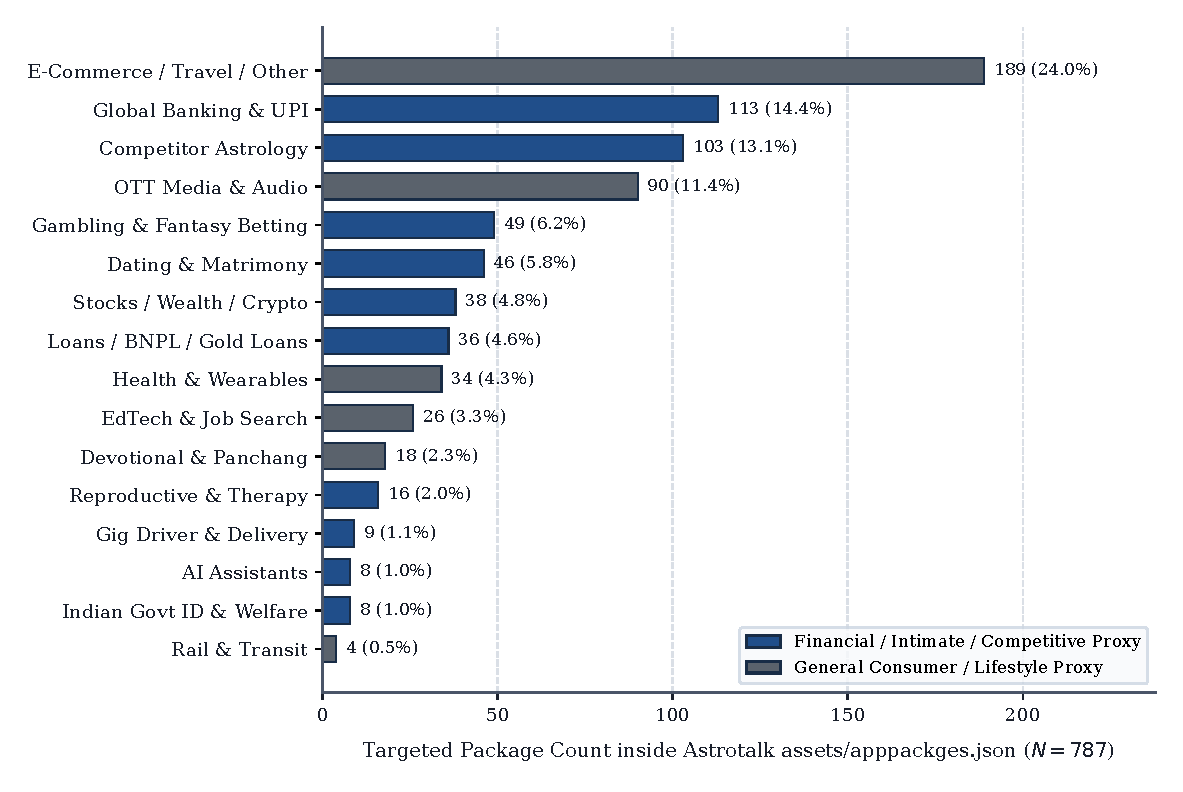
\includegraphics[width=0.90\textwidth]{figures/fig_app_taxonomy.pdf}
\caption{Complete domain distribution across all 787 unique target packages listed in \texttt{Astrotalk.apk} \texttt{assets/apppackges.json}~[sic] (100\% mirrored into manifest \texttt{<queries>}).}
\label{fig:taxonomy}
\end{figure*}

\subsection{Natural Experiment: \texttt{Astrotalk} vs.\ \texttt{Pandit Ji}}
Could \texttt{ExternalPackageTracker} simply be forgotten analytics boilerplate? Comparing \texttt{Astrotalk.apk} directly against its sister app \texttt{Pandit Ji.apk} (\texttt{v1.1.421}) settles that question. Across 7,119 ZIP entries in \texttt{Pandit Ji}, \textbf{6,193 file paths (86.99\%)} overlap with \texttt{Astrotalk}, and \textbf{3,172 files (44.56\%)} have identical uncompressed size and CRC32 checksums. \texttt{Pandit Ji}'s DEX files still contain 1,470 occurrences of the substring \texttt{astrotalk}--spanning live URLs like \url{https://api.astromall.astrotalk.com/AstroMall/}, \url{http://api.kundali.astrotalk.com/v1/}, \url{https://api-kundlireport.astrotalk.in/}, and deep link \nolinkurl{astrotalk://epooja}--alongside \nolinkurl{com.panditji.featureAstroBuddy} DTO classes mirroring \texttt{Astrotalk}'s \url{https://api-astrobuddy.astrotalk.in/}. Yet \texttt{Pandit Ji} contains zero \nolinkurl{assets/apppackges.json}, zero \texttt{ExternalPackageTracker}, zero \nolinkurl{user/apps/installed} route, and only \textbf{26 standard \texttt{<queries>} entries} (UPI PSPs, social sharing, OTPLess, Maps, Chrome). That contrast proves \texttt{Astrotalk}'s 787-app profiler was selectively added and synchronized for the flagship client.

\paragraph{Note on \texttt{AstroSage}, \texttt{Reva}, and \texttt{AstroTime} APKs.}
Neither React Native Hermes APK nor \texttt{AstroSage AI} (\texttt{v32.6}) bundles an installed-app harvester (\texttt{AstroSage}: 23 standard \texttt{<queries>}; \texttt{Reva}: 83; \texttt{AstroTime}: 9). However, \texttt{Reva.apk} requests Android~14's \texttt{DETECT\_SCREEN\_CAPTURE} permission alongside ShareChat subscription endpoints (\nolinkurl{/payments-api-gateway/v1/subscriptions/}, \nolinkurl{revaastro.in}), \texttt{AstroSage AI.apk} retains unencrypted \texttt{http://} endpoints (\url{http://buy.astrosage.com}, \url{http://m2.astrosage.com/compatibility/default.asp}) alongside Razorpay/Paytm/PhonePe SDKs, and \texttt{AstroTime} runs analytics and real-time voice infrastructure over \nolinkurl{apis.theastrotime.com}, \nolinkurl{posthog.theastrotime.com}, and \nolinkurl{cloud-api.livekit.io}.

\subsection{Live Runtime Proxy Verification on Android~14 Lab Emulator}
To verify whether the statically identified upload endpoints execute at runtime without capturing personal user data, we booted an isolated Android~14 Google APIs emulator (\texttt{x86\_64} with \texttt{arm64-v8a} binary translation), installed \texttt{mitmproxy} (\texttt{v12.3.1}) as a System CA inside \nolinkurl{/apex/com.android.conscrypt/cacerts}, installed the unmodified \texttt{Astrotalk} (\texttt{v1.1.545}) split APKs, and tapped \emph{Skip} on onboarding without creating or logging into an account (\nolinkurl{tools/analyze_capture.py}). Across 228 captured HTTP requests, 64 targeted nine \texttt{astrotalk} subdomains (\nolinkurl{api.prod.astrotalk.in}, \nolinkurl{payments-api.astrotalk.in}, \nolinkurl{rudder-prod.astrotalk.in}, \nolinkurl{cdn-exp-api.astrotalk.in}, \nolinkurl{api.astromall.astrotalk.com}, \nolinkurl{api.kundali.astrotalk.com}, \nolinkurl{api.consultant.list.astrotalk.com}, \nolinkurl{aws.astrotalk.com}, and \nolinkurl{astrotalk.com}) with zero TLS pinning rejections. Immediately after dismissing login from \texttt{ChatAstrologer\allowbreak listActivity}, the client fired \texttt{POST} \nolinkurl{https://payments-api.astrotalk.in/AstrotalkPayments/user/save/user-upi-apps} with payload \texttt{\{"upiAppsData":[]\}} (returning HTTP~403 due to unauthenticated guest headers), confirming live execution of UPI-app discovery prior to authentication. By contrast, \texttt{POST} \nolinkurl{user/apps/installed} did not fire during unauthenticated guest browsing, showing that the 787-app catalog check (\texttt{AuthViewModel\$\allowbreak checkExternalPackages}) awaits an authenticated user session.
